\chapter{الحقول الكمومية الموضعية ومعادلة ديراك أحادية البعد}

لقد صادفنا الحقول الكمومية من قبل من خلال كمّاتها، ومؤثرات الإنشاء والإفناء الخاصة بها، وأبسط هاملتوني للجسيمات غير النسبية. وسنجعل هذه الأدوات الآن تؤدي بعض العمل. سنرى أولًا، بدلًا من مجرد الادعاء، كيف يحفظ هاملتوني موضعي مكانيًا الزخم. ثم سندع جداءات الحقول تصف التشتت والاضمحلال، ونراقب كيف يولِّد التأثير المتكرر للهاملتوني بدايات نظرية الاضطراب بالمخططات. وعندئذ فقط سنتجه إلى مسألة الفرميون التي وُعدنا بها. وأوضح مدخل إليها ليس بعدُ حقلاً فرميونيًا، بل معادلة ديراك أحادية البعد.

\section{هاملتوني الحقل مرة أخرى}

يُكتب هاملتوني نوع واحد من الجسيمات غير النسبية على الصورة
\begin{equation}
H_0=\int dx\,
\psi^\dagger(x)
\left[-\frac{\partial_x^2}{2m}+V(x)\right]
\psi(x).
\label{eq:l9-nonrel-hamiltonian}
\end{equation}
وتبدو الكتابة أحادية البعد، لكن لا شيء في الحجة الافتتاحية يعتمد على هذا القيد: ففي ثلاثة أبعاد يمكن أن يدل \(x\) على المتجه \(\mathbf{x}\)، و\(dx\) على \(d^3x\)، و\(-\partial_x^2\) على \(-\nabla^2\).

إن المؤثر \(\psi^\dagger(x)\) ينشئ جسيمًا عند \(x\)، في حين أن \(\psi(x)\) يفنيه هناك. وجداؤهما المرتب ترتيبًا عاديًا
\begin{equation}
n(x)=\psi^\dagger(x)\psi(x)
\end{equation}
هو كثافة العدد الموضعية. ومن ثم يقرأ حد الجهد على الصورة
\begin{equation}
H_V=\int dx\,V(x)n(x).
\end{equation}
وهذا بالضبط ما نكتبه لغاز كلاسيكي: نعدّ الجسيمات القريبة من \(x\)، ونُسنِد إلى كل واحد منها طاقة الوضع \(V(x)\)، ثم نجمع على الفضاء كله. وفي هذه المرحلة لا تتفاعل الجسيمات بعضها مع بعض. وقد تستجيب لجهد مفروض خارجيًا، لكن الهاملتوني فيما عدا ذلك ليس إلا مجموع طاقات أحادية الجسيم مستقلة.

من المفيد أن نُبسِّط أولًا ثم نعكس الاتجاه. فلنأخذ الجهد ثابتًا، \(V(x)=V_0\). فالجهد الثابت لا يؤثر بقوة، لكن معناه المؤثري واضح:
\begin{equation}
\begin{aligned}
H_V&=V_0\int dx\,\psi^\dagger(x)\psi(x)=V_0N,\\
N&=\int dx\,n(x).
\end{aligned}
\end{equation}
إنه يمنح كل جسيم الإضافة الطاقية نفسها. وللاحتفاظ بطاقة السكون في وصف غير نسبي، اختر \(V_0=mc^2\). وعندئذ يعدّ هذا الحد طاقة سكون واحدة لكل جسيم. ونُبقي هذا الثابت، على ما فيه من رتابة في غير ذلك، لأنه يحفظ تناظر الإزاحة ويجعل عملية عدّ الجسيمات ظاهرة.

\section{الهاملتوني بوصفه قاعدة تحديث}

ماذا نعني بقولنا إن الزخم محفوظ؟ ينبغي أن نصوغ الجواب من حيث ما يفعله الهاملتوني. ولكي نتجنب استعمال \(\psi\) في آن واحد لمؤثر حقلي، ولدالة موجية أحادية الجسيم، ولحالة متعددة الأجسام، فلنسمِّ الحالة متعددة الأجسام \(\lvert\Phi(t)\rangle\). وخلال فترة قصيرة \(\epsilon\)،
\begin{equation}
\lvert\Phi(t+\epsilon)\rangle
=\left(1-i\epsilon H+O(\epsilon^2)\right)
\lvert\Phi(t)\rangle,
\label{eq:l9-short-update}
\end{equation}
حيث \(\hbar=1\). تمثل الحالة غير المتغيرة الحد الأول؛ أما أول تصحيح فيولده \(H\). وتكرار هذا التحديث هو معادلة Schr\"odinger.

أصبح حفظ الزخم الآن ذا معنى ملموس. فإذا كانت الحالة الابتدائية ذات زخم كلي محدد \(P\)، فلا بد أن تكون \(H\lvert\Phi\rangle\) ذات الزخم الكلي نفسه. وقد تتغير خواص أخرى، وقد تتبادل الجسيمات المفردة الزخم، لكن لا يجوز للهاملتوني أن ينقل الحالة إلى قطاع يختلف فيه \(P\) الكلي. ويمكننا اختبار ذلك مباشرة بإعادة كتابة الهاملتوني في أساس الزخم.

\section{التكامل المكاني بوصفه دالة دلتا للزخم}

لنختر اصطلاح فورييه
\begin{align}
\psi(x)&=\int\frac{dp}{\sqrt{2\pi}}\,a(p)e^{ipx},\\
\psi^\dagger(x)&=\int\frac{dq}{\sqrt{2\pi}}\,a^\dagger(q)e^{-iqx}.
\label{eq:l9-field-fourier}
\end{align}
يفني المؤثر \(a(p)\) جسيمًا زخمه \(p\).
وينشئ المؤثر \(a^\dagger(q)\) جسيمًا زخمه \(q\). واستخدام حرفين مختلفين أمر أساسي: فالزخمان يُكامل عليهما استقلالًا حتى يربط بينهما التكامل المكاني.

لنبدأ بحد العدد:
\begin{align}
N
&=\int dx\,\psi^\dagger(x)\psi(x)\\
&=\int\frac{dp\,dq}{2\pi}\,
a^\dagger(q)a(p)
\int dx\,e^{i(p-q)x}.
\end{align}
والتكامل المتبقي هو
\begin{equation}
\int dx\,e^{i(p-q)x}=2\pi\delta(p-q).
\end{equation}
عندما يكون \(p\ne q\)، يتذبذب الطور ويلغي نفسه بين الإسهامات الموجبة والسالبة. وعندما يكون \(p=q\)، لا يتذبذب على الإطلاق. وتوزيع دلتا لديراك هو الأداة الدقيقة التي تجمع هاتين الحقيقتين. وبالتالي،
\begin{align}
N
&=\int dp\,dq\,a^\dagger(q)a(p)\delta(p-q)\\
&=\int dp\,a^\dagger(p)a(p).
\label{eq:l9-number-momentum}
\end{align}
يفني هذا المؤثر جسيمًا زخمه \(p\) ويعيد جسيمًا ذا الزخم نفسه تمامًا. وكان العنصر الحاسم هو التكامل على \(x\): إذ أنتج دالة دلتا التي تفرض تساوي الزخم الداخل والزخم الخارج.

\begin{classroomqa}
\lecturetimestamp{00:17:02}
\audiencequestion{ماذا حدث لللانهاية التي تظهر عندما \(p=q\)؟}
\lecturerresponse{لا تُستعمل دالة دلتا بتقييم ارتفاعها. فهي توزيع يُعرَّف بالتكامل: \(\int dk\,\delta(k)f(k)=f(0)\). وعبارة ``مرتفعة إلى ما لا نهاية وضيقة إلى ما لا نهاية'' لا تذكّرنا إلا بأن وزنها التكاملي يساوي واحدًا. وهنا ترشدنا إلى وضع \(p-q=0\)، ولا تبقى أي نتيجة لانهائية.}
\end{classroomqa}

وتعمل الآلية نفسها أيضًا مع حد جدائي موضعي أكثر عمومية بكثير. افترض أن حدًا يحتوي على عدة حقول إفناء وعدة حقول إنشاء، وربما كانت تابعة لأنواع مختلفة، لكن جميعها مُقيَّمة عند نقطة واحدة ويجري التكامل على تلك النقطة:
\begin{equation}
\int dx\,
\prod_{r=1}^{n} \psi_{i_r}^\dagger(x)
\prod_{s=1}^{m} \psi_{j_s}(x).
\end{equation}
ولتكن الجسيمات المُفناة حاملة لزخوم \(p_s\)، والجسيمات المنشأة حاملة لزخوم \(q_r\). عندئذ يعطي تحليل فورييه
\begin{equation}
\int dx\,
e^{i(\sum_s p_s-\sum_r q_r)x}
=2\pi\,
\delta\!\left(\sum_s p_s-\sum_r q_r\right).
\label{eq:l9-total-momentum-delta}
\end{equation}
والنتيجة لا تقرن \(p_1\) بـ \(q_1\)، ولا \(p_2\) بـ \(q_2\)، وهكذا. إنها تفرض فقط
\begin{equation}
\sum_{\mathrm{annihilated}}p
=
\sum_{\mathrm{created}}q.
\end{equation}
وهذه هي بالضبط القاعدة التي يتطلبها التفاعل: فقد تتغير الزخوم المفردة، لكن الزخم الكلي لا يتغير. أما العبارة الأعمق فهي تناظر الإزاحة. فالكثافة الموضعية التي يُكامل عليها بالوزن نفسه عند كل نقطة لا تملك أصلًا مفضلًا، وتحمل تحويلة فورييه الخاصة بها دالة دلتا المناظرة الحافظة للزخم.

\begin{classroomqa}
\lecturetimestamp{00:23:04}
\audiencequestion{هل حد الهاملتوني المقترح هو فعلًا جداء كل تلك المؤثرات الحقلية؟ ولماذا نكتب مثل هذا الجداء؟}
\lecturerresponse{نعم. فهذا الجداء يحدد أي الجسيمات تُفنى وأيها تُنشأ عند نقطة واحدة. وسيأتي دافعه الفيزيائي من عمليات التشتت أو الاضمحلال المرصودة؛ غير أن حجة الزخم تُثبَت أولًا لكي يمكن قراءة تلك التفاعلات مباشرة.}
\end{classroomqa}

\section{الطاقة الحركية في فضاءي الزخم والموضع}

والآن لنطبّق الآلية نفسها على حد المشتقة. تؤثر المشتقة في الموجة المستوية:
\begin{equation}
-\partial_x^2 e^{ipx}=p^2e^{ipx}.
\end{equation}
ولذلك
\begin{align}
H_{\mathrm{kin}}
&=\int dx\,\psi^\dagger(x)
\left(-\frac{\partial_x^2}{2m}\right)\psi(x)\\
&=\int dp\,\frac{p^2}{2m}\,a^\dagger(p)a(p).
\label{eq:l9-kinetic-momentum}
\end{align}
ومرة أخرى يفرض التكامل المكاني تساوي الزخم الداخل والزخم الخارج. أما العامل الجديد \(p^2/2m\) فليس إلا وزنًا لعدد الجسيمات في كل نمط زخمي بطاقة الحركة لذلك النمط.

\begin{classroomqa}
\lecturetimestamp{00:24:46}
\audiencequestion{ألا ينبغي أن يؤدي اشتقاق الموجة المستوية مرتين إلى إشارة سالبة؟}
\lecturerresponse{نعم، \(\partial_x^2e^{ipx}=-p^2e^{ipx}\). ويحتوي الهاملتوني أصلًا على الإشارة السالبة المعوِّضة، لذلك فإن \(-\partial_x^2\) له القيمة الذاتية الموجبة \(p^2\).}
\end{classroomqa}

\begin{classroomqa}
\lecturetimestamp{00:27:20}
\audiencequestion{هل تُحفَظ الطاقة الحركية فقط عندما يكون الجهد ثابتًا؟}
\lecturerresponse{نعم. ففي غياب جهد يعتمد على الموضع لا توجد قوة، وتكون الطاقة الحركية محفوظة على نحو مستقل. أما في جهد خارجي غير ثابت، فيمكن للطاقة الحركية وطاقة الوضع أن تتبادلا، بينما يظل الهاملتوني الكلي محفوظًا إذا لم يعتمد صراحة على الزمن.}
\end{classroomqa}

\begin{classroomqa}
\lecturetimestamp{00:27:42}
\audiencequestion{ما دور \(\psi^\dagger\psi\) في هاملتوني الطاقة الحركية في فضاء الزخم؟}
\lecturerresponse{إنه مؤثر العد. فالجداء النمطي \(a^\dagger(p)a(p)\) يعدّ الجسيمات ذات الزخم \(p\)، ويُسنِد العامل \(p^2/2m\) طاقة الحركة المناسبة إلى كل واحد منها.}
\end{classroomqa}

وثمة طريقة ثانية لرؤية أن هذا الحد غير سالب. فالتكامل بالأجزاء مرة واحدة، مع إهمال حد الحافة، يعطي
\begin{align}
\int dx\,\psi^\dagger(-\partial_x^2)\psi
&=\int dx\,(\partial_x\psi^\dagger)(\partial_x\psi).
\label{eq:l9-positive-kinetic}
\end{align}
وبالنسبة إلى الحقول التي تنعدم على نحو مناسب عند اللانهاية، أو مع شروط حدية دورية، تكون مساهمة الحافة صفرًا. والنتيجة تأخذ صورة مقدار مطلق مربع، ومن ثم فهي غير سالبة. وهي تُظهر أيضًا نمطًا شائعًا في نظرية الحقول: فالطاقة تتضمن مربعات المشتقات المكانية للحقول.

\section{تفاعل تماس موضعي}

لنُسنِد الآن إلى جداءات الحقول مهمة فيزيائية. اعتبر نوعين سنسميهما إلكترونًا وبروتونًا فقط لإبقاء الصورة مألوفة. غير أنهما في الوقت الراهن مزيفان عمدًا: فكلاهما يُعامَل بمؤثرات بوزونية، ويُهمَل تفاعلهما الكولومي الحقيقي. وهاملتونيهما الحر هو
\begin{equation}
H_0=\int dx\left[
\psi_e^\dagger\left(-\frac{\partial_x^2}{2m_e}\right)\psi_e
+
\psi_p^\dagger\left(-\frac{\partial_x^2}{2m_p}\right)\psi_p
\right].
\end{equation}
أضف تفاعل النموذج
\begin{equation}
H_{\mathrm{contact}}
=g\int dx\,
\psi_e^\dagger(x)\psi_p^\dagger(x)
\psi_e(x)\psi_p(x).
\label{eq:l9-contact}
\end{equation}
اقرأه من اليمين إلى اليسار. فهو يبحث عن إلكترون وبروتون عند النقطة نفسها \(x\)، ويفنيهما، ثم يعيد إنشاءهما عند تلك النقطة. وإذا لم يكن الجسيمان معًا، فإن هذا الحد الموضعي يساوي صفرًا. وإذا التقى خطّاهما العالميان، أمكنه أن يغيّر زخميهما الفرديين مع حفظ الزخم الكلي. وهكذا يعمل بوصفه جهد تشتت مثاليًا صفريّ المدى.

\begin{figure}[htbp]
\centering
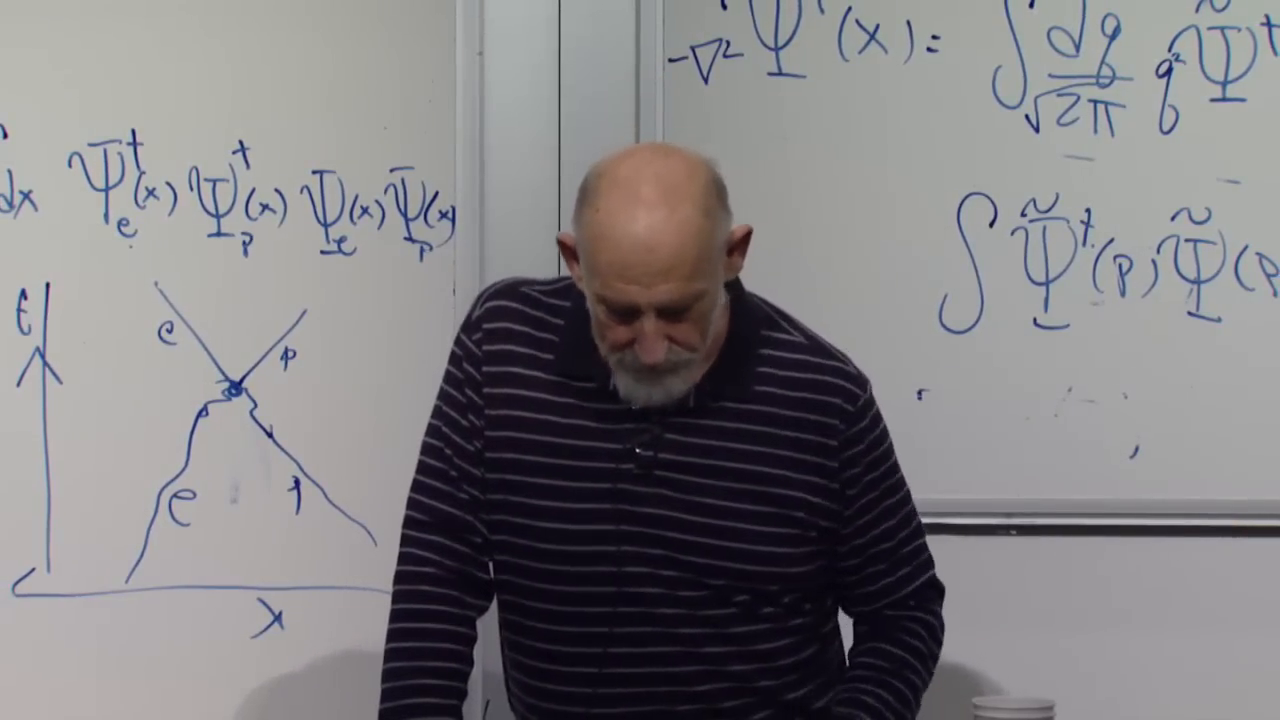
\includegraphics[width=0.94\linewidth]{lecture_09_frame_02.png}
\caption{تفاعل التماس على اللوح. تظهر المؤثرات الحقلية الموضعية الأربعة فوق مخطط الزمكان؛ ونقطة الالتقاء هي الموضع الوحيد الذي يؤثر فيه التفاعل المثالي.}
\lectureframe{00:35:36}
\end{figure}

\begin{figure}[htbp]
\centering
\begin{tikzpicture}[x=1.2cm,y=1.0cm,>=Latex]
\draw[->] (-3.0,0) -- (3.0,0) node[right] {$x$};
\draw[->] (0,-0.2) -- (0,4.2) node[above] {$t$};
\coordinate (v) at (0,2.0);
\fill (v) circle (1.8pt);
\draw[thick,->] (-2.2,0.4) -- (v);
\draw[thick,->] (2.0,0.4) -- (v);
\draw[thick,->] (v) -- (-1.6,3.7);
\draw[thick,->] (v) -- (2.2,3.7);
\node[left] at (-1.65,0.7) {$e$};
\node[right] at (1.55,0.7) {$p$};
\node[left] at (-1.15,3.3) {$e$};
\node[right] at (1.65,3.3) {$p$};
\node[right] at (0.12,2.05) {$g$};
\end{tikzpicture}
\caption{إعادة بناء واضحة لصورة التشتت الموضعي. والرأس اختزال للمؤثر في المعادلة~\eqref{eq:l9-contact}، وليس قانون تصادم كلاسيكيًا.}
\end{figure}

تتفاعل الإلكترونات والبروتونات الحقيقية عن بُعد عبر جهد كولوم. ونموذج التلامس ليس إلا الخطوة الأولى القصيرة: فإذا أظهرت التجربة أن نوعين من الجسيمات يتبعثران فقط عندما يتراكبان، فإن المعادلة~\eqref{eq:l9-contact} هي نوع الحد الذي سنضعه في الهاملتوني.

\begin{classroomqa}
\lecturetimestamp{00:35:40}
\audiencequestion{لماذا يكون مؤثر التبعثر هذا جزءًا من الهاملتوني إذا كانت الطاقة لا تتغير؟}
\lecturerresponse{الهاملتوني هو مؤثر الطاقة، وهو أيضًا المولِّد الذي يغيّر الحالة. فطاقة الوضع بين الجسيمين تُحدث التبعثر تحت التطور الزمني. ولا يعني انحفاظ الطاقة الكلية أن الحالة، أو زخوم الجسيمين كلٌّ على حدة، تبقى بلا تغير.}
\end{classroomqa}

وهذا يعطينا قاعدة عملية. تعلّم أولًا من التجربة ما العمليات الموضعية التي يمكن للجسيمات أن تخضع لها. ثم شفّر تلك العمليات في المؤثر الذي يحدّث الحالة. إن جداءات الحقول ليست جبرًا زخرفيًا: فالعوامل ذات الخناجر والعوامل من دون خناجر تحدد أي الأنواع تظهر وأيها تختفي.

\section{الاضمحلال، والعملية العكسية، والهيرميتية}

لنفترض أن حجرة فقاعات تكشف أثرًا للنوع \(A\) ينتهي عند نقطة تخرج منها آثار \(B\) و\(C\). العملية الموضعية هي
\begin{equation}
A\longrightarrow B+C.
\end{equation}
والمؤثر الذي ينفذها هو
\begin{equation}
V=g\int dx\,
\psi_B^\dagger(x)\psi_C^\dagger(x)\psi_A(x).
\label{eq:l9-decay-half}
\end{equation}
حقل الإفناء يزيل \(A\)؛ وحَقلا الإنشاء يُنتجان \(B\) و\(C\) عند النقطة نفسها. والتكامل بوزن متساوٍ على كل \(x\) يعبّر عن تناظر الانتقال المكاني ويعطي مباشرةً
\begin{equation}
p_A=p_B+p_C.
\end{equation}

يجب أن يكون الهاملتوني هيرميتيًا. وهذا ما يجعل \(e^{-itH}\) وحدويًا ويحفظ الاحتمال الكلي. والمعادلة~\eqref{eq:l9-decay-half} ليست هيرميتية بمفردها، لذلك يجب أن نضيف مرافقها:
\begin{equation}
H_{\mathrm{int}}
=\int dx\left[
g\,\psi_B^\dagger\psi_C^\dagger\psi_A
+g^*\,\psi_A^\dagger\psi_C\psi_B
\right](x).
\label{eq:l9-hermitian-vertex}
\end{equation}
إذا كان الاقتران \(g\) حقيقيًا، فالمعاملان متماثلان. وأخذ المرافق الهيرميتي يعكس ترتيب المؤثرات، فضلًا عن مبادلة الحقول ذات الخناجر بالحقول من دون خناجر. وفي هذا النموذج البوزوني المبسط، تتبادل حقول الأنواع المختلفة، لذلك لا يسبب هذا القلب أي تعقيد إضافي.

والحد الثاني ينفذ العملية العكسية،
\begin{equation}
B+C\longrightarrow A.
\end{equation}
وعليه، فإن هاملتونيًا مغلقًا ووحدويًا يتيح الاضمحلال يحتوي أيضًا على سعة إعادة الاتحاد. وهذا لا يعد بأن كلا الاتجاهين يحدثان لكل مجموعة مختارة من الزخوم الخارجية؛ فقد تجعل الطاقة وقوانين الانحفاظ الأخرى أحد الاتجاهين غير متاح حركيًا. وإنما يعني أن المؤثر ومرافقه كلاهما ينتميان إلى الديناميكيات.

\begin{classroomqa}
\lecturetimestamp{00:42:48}
\audiencequestion{هل يمكن أن يوجد استثناء للقاعدة التي تقضي بأن العملية العكسية مسموح بها أيضًا؟}
\lecturerresponse{ليس على مستوى هاملتوني هيرميتي لنظام مغلق: فالتآثر المرافق مطلوب. وقد يبقى تفاعل عكسي معين محجوبًا بالحركيات أو بعدد كمّي محفوظ آخر، لكن عنصر المصفوفة المرافق موجود.}
\end{classroomqa}

العدد \(g\) هو ثابت الاقتران. فإذا كان \(g\) صغيرًا، فإن الجسيمات التي تلتقي لا تتفاعل إلا تفاعلًا ضعيفًا؛ وإذا كان كبيرًا، كانت سعة الانتقال أكبر. وعادةً ما تكون الاقترانات معاملات تُقاس في التجارب، مع أن التناظرات قد تربط بين عدة اقترانات تبدو مختلفة ظاهريًا.

والنحو نفسه يعالج تفاعلات أشد تعقيدًا. ففي اضمحلال بيتا،
\begin{equation}
n\longrightarrow p+e^-+\bar\nu_e,
\end{equation}
يحتوي حد موضعي تخطيطي على أربعة حقول: أحدها يفني النيوترون، وثلاثة منها تنشئ البروتون والإلكترون وضديد نيوترينو الإلكترون، مع العملية المرافقة هيرميتيًا. وهذا يكفي لرؤية كيف تبدأ مجموعة صغيرة من أحاديات المؤثرات في تعريف نظرية حقل كمومي.

\section{لماذا يهم مربع الهاملتوني}

لقد احتفظت صيغة الزمن القصير \eqref{eq:l9-short-update} بالرتبة الأولى فقط في \(\epsilon\). والتوسع الكامل هو
\begin{equation}
e^{-i\epsilon H}
=1-i\epsilon H-\frac{\epsilon^2}{2}H^2
+\frac{i\epsilon^3}{3!}H^3+\cdots.
\label{eq:l9-exponential}
\end{equation}
وعند الرتبة الثانية يؤثر الهاملتوني مرتين. وهذا هو الأصل الجبري لأول صور العمليات المركبة.

بالنسبة للرأس \(A\leftrightarrow B+C\)، يمكن لفعل واحد أن يجمع \(B+C\) في \(A\)، ويمكن لفعل ثانٍ أن يفكك ذلك \(A\) من جديد إلى \(B+C\):
\begin{equation}
B+C\longrightarrow A\longrightarrow B+C.
\label{eq:l9-bc-scattering}
\end{equation}
والمساهمة الصافية هي سعة تبعثر \(B+C\to B+C\). أما \(A\) الوسيط فليس حدثًا مرصودًا إضافيًا؛ بل يوسم الحالة التي يُجمَع عليها بين فِعْلَي التفاعل.

\begin{classroomqa}
\lecturetimestamp{00:49:54}
\audiencequestion{هل ينبغي أن يحمل حقل \(C\) في الجداء المكتوب من الرتبة الثانية خنجرًا؟}
\lecturerresponse{نعم، يجب أن يطابق ترتيب المؤثرات التسلسل المذكور. فالرأس الأول يفني \(B\) و\(C\) وينشئ \(A\)؛ والثاني يفني \(A\) ويعيد إنشاء \(B\) و\(C\). إن كتابة الخناجر المناظرة على نحو صحيح تعيد هذا التفسير.}
\end{classroomqa}

\begin{figure}[htbp]
\centering
\includegraphics[width=0.94\linewidth]{lecture_09_frame_05.png}
\caption{الاتجاهان للرأس الابتدائي \(A\leftrightarrow B+C\) على اللوح. ووضعهما متجاورين هو الاختزال البصري للعملية من الرتبة الثانية في المعادلة~\eqref{eq:l9-bc-scattering}.}
\lectureframe{00:48:56}
\end{figure}

والآن أضف جسيم \(B\) متفرجًا. يتيح فعل واحد لـ\(A\) أن يصدر \(C\) ويتحول إلى \(B\)؛ ويتيح فعل لاحق لذلك \(C\) أن يتحد مع \(B\) الأصلي ليكوّن \(A\). والجسيمات الخارجية هي من جديد \(A+B\)، لكن زخومها يمكن أن تتغير. ونصف ذلك بأنه تبعثر \(A\) و\(B\) بتبادل \(C\).

\begin{figure}[htbp]
\centering
\includegraphics[width=0.94\linewidth]{lecture_09_frame_06.png}
\caption{بناء التبادل على اللوح. يَصل الرسم الموجود على اليمين بين رأسين ابتدائيين بخط داخلي لـ\(C\) بينما تتبعثر الجسيمات الخارجية \(A\) و\(B\).}
\lectureframe{00:51:22}
\end{figure}

\begin{figure}[htbp]
\centering
\begin{tikzpicture}[x=1.1cm,y=1cm,>=Latex]
\draw[->] (-3.7,-0.2) -- (-3.7,4.2) node[above] {$t$};
\coordinate (v1) at (-0.9,1.25);
\coordinate (v2) at (0.9,2.95);
\fill (v1) circle (1.7pt);
\fill (v2) circle (1.7pt);
\draw[thick,->] (-2.6,0.2) -- (v1) node[midway,below left] {$A$};
\draw[thick,->] (2.6,0.2) -- (v2) node[midway,below right] {$B$};
\draw[thick,->] (v1) -- (-2.4,4.0) node[midway,left] {$B$};
\draw[thick,->] (v2) -- (2.5,4.0) node[midway,right] {$A$};
\draw[thick,->,dashed] (v1) -- (v2) node[midway,above left] {$C$};
\node[below] at (0,-0.05) {$A+B\rightarrow A+B$};
\end{tikzpicture}
\caption{إعادة بناء واضحة لتبادل \(C\). تساهم كل نقطة بعامل واحد من \(g\)، ولذلك يكون هذا الحد من الرتبة الثانية متناسبًا مع \(g^2\).}
\end{figure}

تُسمى كل نقطة تفاعل موضعية رأسًا. ويسهم كل رأس بعامل من اقترانه، لذا تحمل مساهمة ذات رأسين \(g^2\)، وتحمل مساهمة ذات ثلاثة رؤوس \(g^3\)، وهكذا دواليك. ولذلك يربط حد واحد في الهاملتوني بين عائلة كبيرة من التفاعلات. وهذا الاقتصاد هو أحد أسباب قوة نظرية الحقل الكمومي إلى هذا الحد: فعدد صغير من التفاعلات الموضعية ينظم قدرًا هائلًا من بيانات التبعثر.

\begin{classroomqa}
\lecturetimestamp{00:53:14}
\audiencequestion{ماذا نسمي العملية \(A\to B+C\to A\)؟}
\lecturerresponse{إنها مساهمة في الطاقة الذاتية. فـ\(A\) المقاس ليس مجرد حالة الأساس العارية أحادية الجسيم؛ فالحالة المتفاعلة لها أيضًا سعة لمركبات قريبة من \(B+C\). وقد يكشف التبعثر منه تلك البنية الملبَّسة.}
\end{classroomqa}

تقدّم الديناميكا الكهربائية الكمية المثال المألوف. فرأس تآثر موضعي إلكترون--فوتون يمكنه أن يفني إلكترونًا، ويعيد إنشاء إلكترون، وينشئ فوتونًا. وعند الرتبة الثانية، قد يصدر الإلكترون فوتونًا ثم يعيد امتصاصه. ومن المغري أن نروي هذا على أنه فيلم صغير، لكن معناه المنضبط هو حد في التوسع الاضطرابي. والإلكترون الفيزيائي حالة ملبسة ذات مركبات تحتوي فوتونات.

إن التقدير الصفي بأن هذا المركب هو ``حوالي واحد في المئة'' ينقل المقياس الذي يحدده ثابت البنية الدقيقة، \(\alpha_{\mathrm{em}}\simeq 1/137\). ويعتمد احتمال دقيق لمركبة فوتونية في فضاء فوك على دقة الطاقة وعلى الكيفية التي تُعرَّف بها الحالة المتفاعلة؛ وليس خاصية كونية مقدارها واحد في المئة لإلكترون معزول. أما العبارة الراسخة فهي أن التفاعل يغير البنية القابلة للقياس للإلكترون.

\section{ما الذي يقوله المخطط وما الذي لا يقوله}

المخططات اختزال حسابي لقوى هاملتوني التفاعل. وليست تواريخ كلاسيكية موثوقة يؤدي فيها الجسيم حدثًا معينًا ثم آخر على نحو مؤكَّد. إن النظر إلى الداخل لتقرير أي بديل وسيط ``حدث حقًّا'' يغيّر التجربة ويدمر الجمع المتماسك، تمامًا كما في التداخل الكمومي المعتاد.

\begin{classroomqa}
\lecturetimestamp{00:56:52}
\audiencequestion{هل تُحفَظ الطاقة والزخم معًا عند الرأس الأول؟}
\lecturerresponse{في بناء الهاملتوني عند الزمن المتساوي المنفَّذ هنا، ينتج التكامل المكاني فورًا دالة دلتا للزخم. ولم يولد أي تكامل زمني بعدُ دالة دلتا للطاقة لذلك الإدراج المعزول. إن سعة التبعثر الكاملة الثابتة تحت الإزاحة الزمنية تحفظ الطاقة الكلية، في حين لا يلزم للخطوط الوسيطة أن تحقق علاقة على الغلاف الخاصة بالجسيمات المرصودة. وفي لغة المخططات التغايرية تُحفَظ رباعية الزخم عند كل رأس، لكن الجسيمات الداخلية قد تكون خارج الغلاف.}
\end{classroomqa}

إن الطاقة التي تبدو مفقودة في صورة ساذجة للرأس هي تحذير آخر من ألا نهمل طاقة التفاعل. فالهاملتوني الكلي أكثر من مجرد مجموع طاقات الجسيمات الحرة. وإذا نشأ التباس، فارجع إلى المعادلة~\eqref{eq:l9-exponential}: فالصورة تمثل حدًا في توسع التطور الزمني الوحدوي. وتوفر تقنية مخططات فاينمان الكاملة ترتيبًا زمنيًا منهجيًا، ومُنتشرات، وتكاملات، وعوامل تناظر، لكن الفيزياء الأساسية تبدأ هنا.

ويأخذ سؤال مطول المخطط على نحو حرفي أكثر مما ينبغي، إذ يقارن الفوتون المنبعث بالمجال الكهربائي المحيط بإلكترون يتحرك ببطء.

\begin{classroomqa}
\lecturetimestamp{00:58:26}
\audiencequestion{هل المجال الكهربائي للإلكترون على مسافة ما ناتج حرفيًا من فوتونات مشعّة؟ وكيف ينسجم ذلك مع التداخل وتأثير Aharonov--Bohm؟}
\lecturerresponse{الحقل الساكن أو الحقل الحثّي ليس سيلًا من فوتونات مشعّة حقيقية. تصف الكهروديناميكا الكمومية كلًا من الإشعاع وكساء الإلكترون الكهرومغناطيسي بالحقل نفسه، لكن الحالات الكمومية والحركيات المقابلة تختلف. بالنسبة إلى إلكترون فائق النسبية، يمكن لبعض مركبات الحقل أن تتصرف، على نحو مفيد، كدفق من فوتونات شبه حقيقية؛ أمّا بالنسبة إلى إلكترون بطيء، فإن نموذج مسار فوتون حرفي هو النموذج الخاطئ. كما أن تداخل الشقين وتأثير Aharonov--Bohm ظاهرتان حقليتان لا كلاسيكيتان أيضًا، لكنهما لا يحولان مخطط الطاقة الذاتية هذا إلى فيلم ميكانيكي.}
\end{classroomqa}

\begin{classroomqa}
\lecturetimestamp{01:01:28}
\audiencequestion{لماذا يفشل بالضبط نموذج كلاسيكي لهذا المخطط؟}
\lecturerresponse{لأن الحساب يجمع على نحو مترابط سعات جميع البدائل الوسيطة المسموح بها. تجعل الخبرة هذه الصور مألوفة حدسيًا، لكن محتواها الحرفي لا يتجاوز أبدًا التوسع المؤثري الذي يعرّفها. إنها طريقة مدمجة لحساب \(H^2,H^3,\ldots\)، وليست سجلًا لأحداث وسيطة مُشاهدة.}
\end{classroomqa}

\begin{classroomqa}
\lecturetimestamp{01:03:04}
\audiencequestion{هل يمكن أن ينشأ تآثر كولوم المعتاد بوصفه الحد الكلاسيكي لتبادل الفوتونات؟}
\lecturerresponse{نعم. إن تقييم السعة المناسبة المتوسطة بفوتون وأخذ النهاية الساكنة غير النسبية يعطيان كمون كولوم. والاشتقاق أكثر تقنية من هذا التخطيط المؤثري الحالي، ومع ذلك لا ينبغي أن يُقرأ على أنه فوتون يقفز حرفيًا بين جسيمين كلاسيكيين.}
\end{classroomqa}

\begin{classroomqa}
\lecturetimestamp{01:03:44}
\audiencequestion{هل تُحسب ثوابت الاقتران من جداءات الحقول؟}
\lecturerresponse{تكون قيمها العددية عادةً مُدخلات تجريبية. ويمكن للتناظر أن يقيّدها أو يربط بين اقترانات كانت ستبقى مستقلة لولا ذلك. وعندما تتنبأ مثل هذه العلاقة بالشدد النسبية لتفاعلات متميزة ويؤكدها التجريب، يكون هذا التوافق ذا دلالة خاصة.}
\end{classroomqa}

\begin{classroomqa}
\lecturetimestamp{01:04:48}
\audiencequestion{ما دور التناظر العرضي مقارنةً بالتناظر المعياري؟}
\lecturerresponse{يقيّد التناظر المعياري مباشرة البنية المسموح بها والعلاقات بين الاقترانات. أمّا التناظر العرضي فلا يُفرض على المستوى الأساسي، بل يظهر لأن جميع التفاعلات المسموح بها من الرتبة الأدنى تصادف أنها تحترمه. ومع ذلك يمكن أن تترتب عليه نتائج مهمة، مع أن أصله ومتانته يختلفان عن أصل التناظر المعياري ومتانته.}
\end{classroomqa}

هذا يكفي من نظرية الحقول غير النسبية في الوقت الحاضر. لقد وعدنا بالفرميونات. وبدلًا من أن نكممها تكميمًا ثانيًا مباشرة، سنفهم أولًا معادلة الجسيم الواحد النسبية التي يجب أن تحققها مؤثرات حقولها.

\section{لماذا يحتاج الإلكترون إلى النسبية}

ابدأ في بعد مكاني واحد. هذا ليس قيدًا واقعيًا، لكنه يزيل التعقيد الهندسي للسبين في ثلاثة أبعاد مع الحفاظ على الجبر الأساسي. كتلة الإلكترون صغيرة بما يكفي بحيث تصبح النسبية مهمة حتى في الذرات. ففي الهيدروجين تكون سرعته المميزة من رتبة
\begin{equation}
v\sim\alpha_{\mathrm{em}}c\approx 0.007c,
\end{equation}
أي قرابة واحد في المئة من سرعة الضوء. أمّا بالنسبة إلى الإلكترونات الداخلية في ذرة ثقيلة، فيصبح المقياس التقريبي \(v\sim Z\alpha_{\mathrm{em}}c\)، ولذلك قد تكون التصحيحات النسبية كبيرة. وسواء أكان الدافع الحاسم فضولًا تاريخيًا أم دقةً ذرية، فإن معادلة نسبية شبيهة بمعادلة Schr\"odinger ضرورية فيزيائيًا.

تبدأ الوصفة المعتادة للتكميم من العلاقة الكلاسيكية بين الطاقة والزخم. ففي الحالة غير النسبية،
\begin{equation}
E=\frac{p^2}{2m},
\end{equation}
وتؤدي الإحلالات
\begin{equation}
E\mapsto i\partial_t,
\qquad
p\mapsto-i\partial_x
\end{equation}
إلى
\begin{equation}
i\partial_t\varphi(x,t)
=-\frac{1}{2m}\partial_x^2\varphi(x,t).
\end{equation}

أمّا النسبية فتعطي، مع \(c=1\)،
\begin{equation}
E^2=p^2+m^2.
\label{eq:l9-rel-dispersion}
\end{equation}

\begin{figure}[htbp]
\centering
\includegraphics[width=0.94\linewidth]{lecture_09_frame_07.png}
\caption{الانتقال على اللوح من \(E=p^2/2m\) إلى العلاقة النسبية \(E^2=p^2+m^2\)، مع \(c=1\).}
\lectureframe{01:10:30}
\end{figure}

يؤدي تطبيق الإحلالات على العلاقة المربعة إلى
\begin{equation}
-\partial_t^2\varphi
=\left(-\partial_x^2+m^2\right)\varphi,
\label{eq:l9-klein-gordon}
\end{equation}
أو على نحو مكافئ
\begin{equation}
\left(\partial_t^2-\partial_x^2+m^2\right)\varphi=0.
\end{equation}
هذه هي معادلة Klein--Gordon. إنها معادلة حقل نسبية ذات معنى تام، ولا سيما لحقول السبين الصفري. لكن المعادلة المنشودة للإلكترون يجب أن تكون من الرتبة الأولى في الزمن،
\begin{equation}
i\partial_t\Psi=H\Psi,
\end{equation}
بحيث يولّد \(H\) نفسه، لا \(H^2\) فقط، التطور.

يمكن صوريًا أن نختار
\begin{equation}
H=\sqrt{-\partial_x^2+m^2}.
\end{equation}
يمكن تعريف الجذر التربيعي على نحو نظيف في فضاء الزخم، حيث يعمل بالضرب في \(\sqrt{p^2+m^2}\)، لكنه في فضاء الموضع مؤثر شبه تفاضلي لاموضعي. وهو ذو معنى تقني، لكنه غير مساعد من الناحية الجمالية للمعادلة الموضعية التي نبحث عنها. لذلك نبدأ من جديد.

\section{موجة عديمة الكتلة تسير إلى اليمين}

لنأخذ أولًا جسيمًا عديم الكتلة يتحرك إلى اليمين. تحقق طاقته الموجبة وزخمه
\begin{equation}
E=p
\qquad (c=1).
\end{equation}
ويعطي التكميم
\begin{equation}
i\partial_t\psi=-i\partial_x\psi,
\end{equation}
أو
\begin{equation}
(\partial_t+\partial_x)\psi=0.
\label{eq:l9-right-mover}
\end{equation}
وكل حل له الشكل
\begin{equation}
\psi(x,t)=f(x-t).
\end{equation}
ويبقى الشكل ثابتًا ويتحرك إلى اليمين بسرعة الضوء.

تظهر صعوبتان فورًا. أولًا، إذا سُمِح للمعادلة~\eqref{eq:l9-right-mover} أن تعمل على أنماط فورييه الاعتباطية، فللزخم السالب طاقة \(E=p<0\)، ولذلك لا يملك الهاملتوني حدًا أدنى. إن تقييدها يدويًا إلى \(p>0\) لا يُبقي إلا المتحركات إلى اليمين، وليس بعدُ نظرية الإلكترون التي نريدها. ثانيًا، المعادلة طريق في اتجاه واحد: فهي لا تحتوي على إلكترون عادي يتحرك إلى اليسار. سنعالج مشكلة اليمين واليسار أولًا ونترك الطاقات السالبة على حالها.

\section{مركبتان ومصفوفة ألفا}

أدخل سعتين،
\begin{equation}
\Psi(x,t)=
\begin{pmatrix}
\psi_1(x,t)\\[3pt]
\psi_2(x,t)
\end{pmatrix},
\end{equation}
حيث تكون \(\psi_1\) متحركة إلى اليمين وتكون \(\psi_2\) متحركة إلى اليسار في الحد العديم الكتلة:
\begin{align}
(\partial_t+\partial_x)\psi_1&=0,
&
(\partial_t-\partial_x)\psi_2&=0.
\end{align}
وتسمح ميكانيكا الكم أيضًا بتراكبات اعتباطية من الاثنتين. لذلك يمكن للجسيم أن يمتلك سعات لكلا الاتجاهين بدلًا من أن يحمل وسمًا كلاسيكيًا يُختار مرة واحدة وإلى الأبد.

تشبه درجة الحرية الإضافية الثنائية القيم السبين من حيث الجبر، لكنها في بعد واحد ليست عزمًا زاويًا عاديًا. عرّف
\begin{equation}
\alpha=
\begin{pmatrix}
1&0\\
0&-1
\end{pmatrix}
=\sigma_3.
\label{eq:l9-alpha}
\end{equation}
فالمتجه الذاتي الموافق لـ \(+1\) ينتقي المركبة المتحركة إلى اليمين، والمتجه الذاتي الموافق لـ \(-1\) ينتقي المركبة المتحركة إلى اليسار. وفي النظرية عديمة الكتلة يكون الهاملتوني ببساطة
\begin{equation}
H=\alpha p,
\end{equation}
وتجتمع المعادلتان في
\begin{equation}
i\partial_t\Psi=-i\alpha\partial_x\Psi.
\label{eq:l9-massless-dirac}
\end{equation}

\begin{classroomqa}
\lecturetimestamp{01:22:44}
\audiencequestion{ما اسم المصفوفة القطرية التي تميّز بين المركبتين؟}
\lecturerresponse{بوصفها مصفوفة باولي فهي \(\sigma_3\)، لا \(\sigma_1\). وفي ترميز ديراك لهذا البناء الحالي نسميها \(\alpha\). وجبرها هو جبر باولي المألوف، مع أن الوسم الفيزيائي هنا هو الاتجاه لا العزم الزاوي المغزلي.}
\end{classroomqa}

\begin{classroomqa}
\lecturetimestamp{01:23:32}
\audiencequestion{هل يكتسب هذا البناء معنىً هندسيًا أكثر في ثلاثة أبعاد، حيث يكون الاتجاه متجهًا؟}
\lecturerresponse{نعم. تتطلب المسألة ثلاثية الأبعاد مصفوفة لكل اتجاه مكاني، وتؤدي إلى بنية سبينورية أغنى. ومع ذلك فإن النموذج أحادي البعد دقيق تمامًا ضمن إطاره الخاص، ويعزل جبر اليمين واليسار الأساسي من دون ذلك التعقيد الإضافي.}
\end{classroomqa}

\begin{figure}[htbp]
\centering
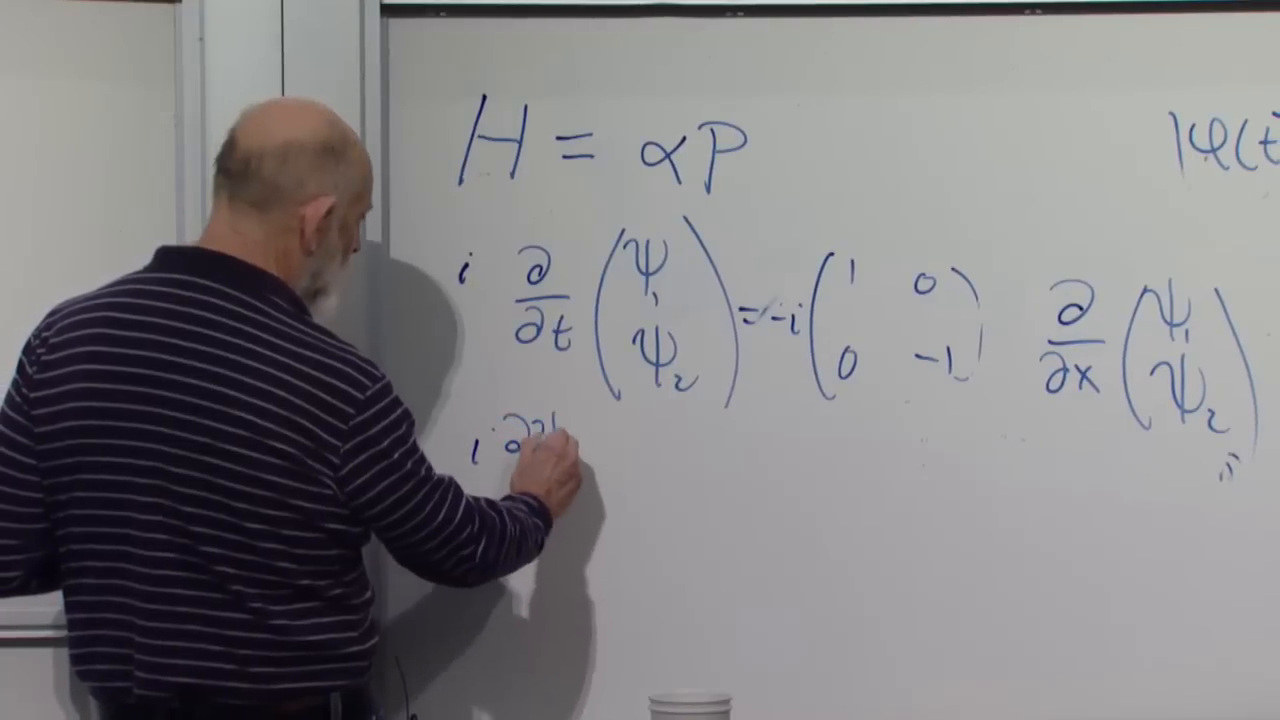
\includegraphics[width=0.94\linewidth]{lecture_09_frame_03.png}
\caption{معادلة المركبتين عديمة الكتلة على اللوح: \(H=\alpha P\)، حيث تسند المصفوفة القطرية انتشارًا متعاكسًا إلى \(\psi_1\) و\(\psi_2\).}
\lectureframe{01:26:00}
\end{figure}

زالت مشكلة الاتجاه الواحد. ويبقى طيف الطاقات السالبة، وقد اكتشفنا عيبًا ثالثًا: فما تزال المركبتان عديمتي الكتلة وتنتشران بسرعة الضوء. ولا بد في الخطوة التالية من إدخال طاقة سكون والاقتران بين الاتجاهين.

\section{إضافة الكتلة واكتشاف جبر ديراك}

أضف أبسط حد عام متناسب مع الكتلة،
\begin{equation}
H=\alpha p+\beta m,
\label{eq:l9-dirac-hamiltonian}
\end{equation}
حيث يعمل \(\beta\) فقط على المؤشر ذي المركبتين. وكان يمكن أن يكون مصفوفة الوحدة أو مصفوفة أخرى؛ ونَدَع علاقة التشتت النسبية تحسم ذلك.

بما أن \(H^2\) يجب أن يساوي \(p^2+m^2\)، فلنربع المعادلة~\eqref{eq:l9-dirac-hamiltonian}:
\begin{align}
H^2
&=(\alpha p+\beta m)^2\\
&=\alpha^2p^2+\beta^2m^2
+(\alpha\beta+\beta\alpha)pm.
\label{eq:l9-square-dirac}
\end{align}
تتبادل المصفوفات مع \(p\) لأنّها تؤثر في الحيز الداخلي ذي المركبتين، بينما يؤثر \(p\) في الدالة الموجية المكانية. ومطابقة المعادلة~\eqref{eq:l9-rel-dispersion} تستلزم
\begin{equation}
\alpha^2=\mathbb{1},
\qquad
\beta^2=\mathbb{1},
\qquad
\{\alpha,\beta\}
=\alpha\beta+\beta\alpha=0.
\label{eq:l9-dirac-algebra}
\end{equation}
الشرط الأول متحقق أصلًا من أجل \(\alpha=\sigma_3\). وأي مصفوفة باولي أخرى تحقق معها ضد التبادل، ومربعها يساوي مصفوفة الوحدة. اختر
\begin{equation}
\beta=
\begin{pmatrix}
0&1\\
1&0
\end{pmatrix}
=\sigma_1.
\label{eq:l9-beta}
\end{equation}
واختيار \(\sigma_1\) بدلًا من \(\sigma_2\) هو اصطلاح للأساس؛ فكلاهما يحقق الجبر نفسه بعد تغيير وحدوي للأساس.

\begin{classroomqa}
\lecturetimestamp{01:33:00}
\audiencequestion{هل أدرك ديراك ببساطة أن مصفوفات باولي تحقق هذه الشروط الجبرية؟}
\lecturerresponse{أُجري الاشتقاق التاريخي مباشرة في ثلاثة أبعاد، وأُدخلت فيه مصفوفات تحقق العلاقات المطلوبة. وبمجرد أن تُكتب الشروط، يجعل جبر باولي الحل في بعد واحد فوريًا: اختر مصفوفتين مختلفتين من مصفوفات باولي.}
\end{classroomqa}

\begin{classroomqa}
\lecturetimestamp{01:34:24}
\audiencequestion{هل هذا \(\beta\) هو معامل السرعة النسبي \(v/c\)؟}
\lecturerresponse{لا. بل هو مصفوفة تؤثر في مكوّنات السبينور. والحرف المعاد استخدامه ليس إلا ترميز ديراك؛ ولا علاقة له بالكمية الحركية \(v/c\).}
\end{classroomqa}

في ثلاثة أبعاد مكانية، لا تكفي مصفوفات \(2\times2\) للمجموعة الكاملة المطلوبة من المصفوفات المتضادة التبادل. ويُؤجَّل هذا التوسيع. وفي بُعد واحد، تكفي المعادلتان ~\eqref{eq:l9-alpha} و\eqref{eq:l9-beta}.

\section{معادلة ديراك المقترنة في بُعد واحد}

وبالتعويض بـ\(p=-i\partial_x\) نحصل على معادلة ديراك في بُعد واحد بصيغة هاملتونية:
\begin{equation}
i\partial_t\Psi
=\left(-i\alpha\partial_x+\beta m\right)\Psi.
\label{eq:l9-one-dimensional-dirac}
\end{equation}
ولأن \(\alpha\) قطرية، فإن حدَّ المشتقة المرتبط بها يُبقي المركبتين منفصلتين. ولأن \(\beta\) خارج القطر، فإن حدَّ الكتلة يبدّل إحداهما بالأخرى. وعند كتابتها مركبةً فمركبةً،
\begin{align}
i\partial_t\psi_1
&=-i\partial_x\psi_1+m\psi_2,
\label{eq:l9-dirac-component-one}\\
i\partial_t\psi_2
&=+i\partial_x\psi_2+m\psi_1.
\label{eq:l9-dirac-component-two}
\end{align}

\begin{figure}[htbp]
\centering
\includegraphics[width=0.94\linewidth]{lecture_09_frame_08.png}
\caption{معادلتا المركبتين المقترنتان على اللوح. تُرمِّز إشارتا المشتقة المتعاكستان إلى الحركة نحو اليمين ونحو اليسار؛ وحدُّ الكتلة خارج القطر يبدّل بين \(\psi_1\) و\(\psi_2\).}
\lectureframe{01:37:44}
\end{figure}

لا تعود المركبتان تتطوران على نحو مستقل ما إن \(m\ne0\). ومن تربيع المعادلة من الرتبة الأولى نستعيد مؤثر كلاين--غوردون على كل مركبة،
\begin{equation}
\left(\partial_t^2-\partial_x^2+m^2\right)\psi_a=0,
\qquad a=1,2,
\end{equation}
وتحقق الموجات المستوية \(E^2=p^2+m^2\). وتكون سرعتها الزمرية
\begin{equation}
v_g=\frac{dE}{dp}=\frac{p}{E},
\end{equation}
ويكون مقدارها أقل من الواحد عند كتلة غير منعدمة.

العلاقة بين الكتلة والخلط بين اليسار واليمين ليست مصادفة. فالمتحرك العديم الكتلة إلى اليمين يبقى متحركًا إلى اليمين تحت كل تعزيز لورنتزي صحيح؛ ولا يستطيع أي راصد دون ضوئي أن يسبق الضوء ويعكس اتجاهه. أما الجسيم ذو الكتلة فيمكن الإتيان به إلى السكون ثم النظر إليه من إطار أسرع يتحرك في الاتجاه نفسه، حيث تبدو سرعته معكوسة. ولذلك لا يمكن لنظرية نسبية ذات كتلة أن تُبقي قطاعي اليمين واليسار معزولين على الدوام. وحدُّ الكتلة خارج القطر يوفّر بالضبط الاقتران المطلوب.

\begin{classroomqa}
\lecturetimestamp{01:40:01}
\audiencequestion{هل يُعدّ تبديل المركبتين تذبذبًا كيراليًا؟}
\lecturerresponse{في هذا الأساس أحادي البعد، يميّز \(\alpha\) بين الاتجاهين الكيراليين في الحالة عديمة الكتلة. وحدُّ الكتلة خارج القطر يمزجهما، لذا لم تعد الكيرالية محفوظة. وبهذا المعنى فإن حدَّ الكتلة هو مصدر التذبذب الكيرالي.}
\end{classroomqa}

\begin{classroomqa}
\lecturetimestamp{01:40:46}
\audiencequestion{لماذا ينبغي أن تكون معادلة فرميون الجذر التربيعي لمعادلة بوزونية؟}
\lecturerresponse{لا ينبغي فهم الأمر على هذا النحو. فعلاقة التشتت \(E^2=p^2+m^2\) تنطبق على كل جسيم حر نسبي، بصرف النظر عن الإحصاء. ويصادف أن مؤثر ديراك يوفّر تحليلاً مصفوفيًا لمؤثر كلاين--غوردون، لكن تلك العلاقة الجبرية لا تشتق الفرميونات من البوزونات.}
\end{classroomqa}

\begin{classroomqa}
\lecturetimestamp{01:41:31}
\audiencequestion{هل يمكن اختزال المعادلة إلى تحليل قياسي بسيط إلى عاملين منفصلين، أحدهما للحركة نحو اليسار والآخر للحركة نحو اليمين؟}
\lecturerresponse{فقط في حد انعدام الكتلة تنفصل المعادلتان الكيراليتان إلى عاملين قياسيين مستقلين. أما عندما \(m\ne0\)، فإن التحليل المفيد يكون مصفوفيًا: فمصفوفتا \(\alpha\) و\(\beta\) المتضادتان في التبادل هما اللتان تزيلان الحد المتقاطع غير المرغوب فيه.}
\end{classroomqa}

\begin{classroomqa}
\lecturetimestamp{01:42:04}
\audiencequestion{هل تشكل هاتان المعادلتان المقترنتان بالفعل معادلة ديراك؟}
\lecturerresponse{نعم. فهما معًا تمثلان معادلة ديراك في بُعد مكاني واحد، ويمكن كتابتهما بصورة مكافئة في الصيغة الموجزة للمعادلة ~\eqref{eq:l9-one-dimensional-dirac}. ويمكن الحصول على تدوين تغايري أكثر تناظرًا بالضرب في \(\beta\)، لكن يُؤجَّل تقديم ذلك الشكل.}
\end{classroomqa}

تبقى مهمتان غير منجزتين عمدًا. فهذا البناء لم يزل الطاقات السالبة؛ بل أعطى حلولًا سالبة الطاقة في كلا القطاعين الاتجاهيين، ولذلك أصبحت تلك المشكلة الآن أشد بروزًا لا أقل. وما تزال النظرية تعيش في بُعد مكاني واحد. والخطوتان التاليتان هما تفسير حلول الطاقة السالبة وتوسيع جبر المصفوفات إلى أبعاد \(3+1\).
